\newcommand{\customDir}{}
\RequirePackage{ifthen,xifthen}

% Input inkl. Umlaute, Silbentrennung
\RequirePackage[T1]{fontenc}
\RequirePackage[utf8]{inputenc}

% Arbeitsordner (in Abhängigkeit vom Master) Standard: .LateX_master Ordner liegt im Eltern-Ordner
\providecommand{\customDir}{../}
\newcommand{\setCustomDir}[1]{\renewcommand{\customDir}{#1}}
%%% alle Optionen:
% Doppelseitig (mit Rand an der Innenseite)
\newboolean{twosided}
\setboolean{twosided}{false}
% Eigene Dokument-Klasse (alle KOMA möglich; cheatsheet für Spicker [3 Spalten pro Seite, alles kleiner])
\newcommand{\customDocumentClass}{scrreprt}
\newcommand{\setCustomDocumentClass}[1]{\renewcommand{\customDocumentClass}{#1}}
% Unterscheidung verschiedener Designs: htw, fjs
\newcommand{\customDesign}{htw}
\newcommand{\setCustomDesign}[1]{\renewcommand{\customDesign}{#1}}
% Dokumenten Metadaten
\newcommand{\customTitle}{}
\newcommand{\setCustomTitle}[1]{\renewcommand{\customTitle}{#1}}
\newcommand{\customSubtitle}{}
\newcommand{\setCustomSubtitle}[1]{\renewcommand{\customSubtitle}{#1}}
\newcommand{\customAuthor}{}
\newcommand{\setCustomAuthor}[1]{\renewcommand{\customAuthor}{#1}}
%	Notiz auf der Titelseite (A: vor Autor, B: nach Autor)
\newcommand{\customNoteA}{}
\newcommand{\setCustomNoteA}[1]{\renewcommand{\customNoteA}{#1}}
\newcommand{\customNoteB}{}
\newcommand{\setCustomNoteB}[1]{\renewcommand{\customNoteB}{#1}}
% Format der Signatur in Fußzeile:
\newcommand{\customSignature}{\ifthenelse{\equal{\customAuthor}{}} {} {\footnotesize{\textcolor{darkgray}{Mitschrift von\\ \customAuthor}}}}
\newcommand{\setCustomSignature}[1]{\renewcommand{\customSignature}{#1}}
% Format des Autors auf dem Titelblatt:
\newcommand{\customTitleAuthor}{\textcolor{darkgray}{Mitschrift von \customAuthor}}
\newcommand{\setCustomTitleAuthor}[1]{\renewcommand{\customTitleAuthor}{#1}}
% Standard Sprache
\newcommand{\customDefaultLanguage}[1]{}
\newcommand{\setCustomDefaultLanguage}[1]{\renewcommand{\customDefaultLanguage}{#1}}
% Folien-Pfad (inkl. Dateiname ohne Endung und ggf. ohne Nummerierung)
\newcommand{\customSlidePath}{}
\newcommand{\setCustomSlidePath}[1]{\renewcommand{\customSlidePath}{#1}}
% Folien Eigenschaften
\newcommand{\customSlideScale}{0.5}
\newcommand{\setCustomSlideScale}[1]{\renewcommand{\customSlideScale}{#1}}

%\setboolean{twosided}{true}
%\setCustomDocumentClass{scrartcl}
%\setCustomDesign{htw}
\setCustomSlidePath{Vorlesung/VO}
\setCustomSlideScale{1.5}

\setCustomTitle{Software Engineering 1}
\setCustomSubtitle{Beleg}
\setCustomAuthor{Falk-Jonatan Strube}
%\setCustomNoteA{TitlepageNoteBeforeAuthor}
\setCustomNoteB{Vorlesung von Prof. Dr. Hauptmann}

\setCustomSignature{\footnotesize{\textcolor{darkgray}{von Luga, Pour, \\Retsch, Strube}}}	% Formatierung der Signatur in der Fußzeile
\setCustomTitleAuthor{\textcolor{darkgray}{\customAuthor}}	% Formatierung des Autors auf dem Titelblatt

%-- Prüfen, ob Beamer
\ifthenelse{\equal{\customDocumentClass}{beamer}}{
%%% TODO: andere Layouts für Beamer außer HTW
	\documentclass[ignorenonframetext, 11pt, table]{beamer}
	
	\usenavigationsymbolstemplate{}
	\setbeamercolor{author in head/foot}{fg=black}
	\setbeamercolor{title}{fg=black}
	\setbeamercolor{bibliography entry author}{fg=htworange!70}
	%\setbeamercolor{bibliography entry title}{fg=blue} 
	\setbeamercolor{bibliography entry location}{fg=htworange!60} 
	\setbeamercolor{bibliography entry note}{fg=htworange!60}  
	
	\setbeamertemplate{itemize item}{\color{black}$\bullet$}
	\setbeamertemplate{itemize subitem}{\color{black}--}
	\setbeamertemplate{itemize subsubitem}{\color{black}$\bullet$}
	\makeatother
	\setbeamertemplate{footline}
	{
	\leavevmode
	\def\arraystretch{1.2}
	\arrayrulecolor{gray}
	\begin{tabular}{ p{0.167\textwidth} | p{0.491\textwidth} | p{0.089\textwidth} | p{0.103\textwidth}}
	\hline
	\strut\insertshortauthor & \insertshorttitle & Slide \insertframenumber{}% / \inserttotalframenumber{}
	 & May 4, 2016\\
	\end{tabular}
	}
	\setbeamertemplate{headline}
	{
	\leavevmode
	\setlength{\arrayrulewidth}{1pt}
	\hspace*{2em}	
	\begin{tabular}{p{0.63\textwidth}}
	\rule{0pt}{3em}\normalsize{\textbf{\insertsection\strut}}\\
	\arrayrulecolor{htworange}
	\hline
	\end{tabular}
	\begin{tabular}{l}
	\rule{0pt}{4em}\includegraphics[width=3.25cm]{\customDir _LaTeX_master/HTW_GESAMTLOGO_CMYK.eps}\\
	\end{tabular}
	}
	\makeatletter	
}{	
	%-- Für Spicker einiges anders:
	\ifthenelse{\equal{\customDocumentClass}{cheatsheet}}{
		\documentclass[a4paper,10pt,landscape]{scrartcl}
		\usepackage{geometry}
		\geometry{top=2mm, bottom=2mm, headsep=0mm, footskip=0mm, left=2mm, right=2mm}
		
		% Für Spicker \spsection für Section, zur Strukturierung \HRule oder \HDRule Linie einsetzen
		\usepackage{multicol}
		\newcommand{\spsection}[1]{\textbf{#1}}	% Platzsparende "section" für Spicker
	}{	%-- Ende Spicker-Unterscheidung-if
		%-- Unterscheidung Doppelseitig
		\ifthenelse{\boolean{twosided}}{
			\documentclass[a4paper,11pt, footheight=26pt,twoside]{\customDocumentClass}
			\usepackage[head=23pt]{geometry}	% head=23pt umgeht Fehlerwarnung, dafür größeres "top" in geometry
			\geometry{top=30mm, bottom=22mm, headsep=10mm, footskip=12mm, inner=27mm, outer=13mm}
		}{
			\documentclass[a4paper,11pt, footheight=26pt]{\customDocumentClass}
			\usepackage[head=23pt]{geometry}	% head=23pt umgeht Fehlerwarnung, dafür größeres "top" in geometry
			\geometry{top=30mm, bottom=22mm, headsep=10mm, footskip=12mm, left=20mm, right=20mm}
		}
		%-- Nummerierung bis Subsubsection für Report
		\ifthenelse{\equal{\customDocumentClass}{report} \OR \equal{\customDocumentClass}{scrreprt}}{
			\setcounter{secnumdepth}{3}	% zählt auch subsubsection
			\setcounter{tocdepth}{3}	% Inhaltsverzeichnis bis in subsubsection
		}{}
	}%-- Ende Spicker-Unterscheidung-else
	
	\usepackage{scrlayer-scrpage}	% Kopf-/Fußzeile
	\renewcommand*{\thefootnote}{\fnsymbol{footnote}}	% Fußnoten-Symbole anstatt Zahlen
	\renewcommand*{\titlepagestyle}{empty} % Keine Seitennummer auf Titelseite
	\usepackage[perpage]{footmisc}	% Fußnotenzählung Seitenweit, nicht Dokumentenweit
}

% Input inkl. Umlaute, Silbentrennung
\RequirePackage[T1]{fontenc}
\RequirePackage[utf8]{inputenc}
\usepackage[english,ngerman]{babel}
\usepackage{csquotes}	% Anführungszeichen
\RequirePackage{marvosym}
\usepackage{eurosym}

% Style-Aufhübschung
\usepackage{soul, color}	% Kapitälchen, Unterstrichen, Durchgestrichen usw. im Text
%\usepackage{titleref}
\usepackage[breakwords, fit]{truncate}	% Abschneiden von Sätzen
\renewcommand{\TruncateMarker}{\,…}

% Mathe usw.
\usepackage{amssymb}
\usepackage{amsthm}
\ifthenelse{\equal{\customDocumentClass}{beamer}}{}{
\usepackage[fleqn,intlimits]{amsmath}	% fleqn: align-Umgebung rechtsbündig; intlimits: Integralgrenzen immer ober-/unterhalb
}
%\usepackage{mathtools} % u.a. schönere underbraces
\usepackage{xcolor}
\usepackage{esint}	% Schönere Integrale, \oiint vorhanden
\everymath=\expandafter{\the\everymath\displaystyle}	% Mathe Inhalte werden weniger verkleinert
\usepackage{wasysym}	% mehr Symbole, bspw \lightning
%\renewcommand{\int}{\int\limits}
%\usepackage{xfrac}	% mehr fracs: sfrac{}{}
\let\oldemptyset\emptyset	% schöneres emptyset
\let\emptyset\varnothing
%\RequirePackage{mathabx}	% mehr Symbole
\mathchardef\mhyphen="2D	% Hyphen in Math

% tikz usw.
\usepackage{tikz}
\usepackage{pgfplots}
\pgfplotsset{compat=1.11}	% Umgeht Fehlermeldung
\usetikzlibrary{graphs}
%\usetikzlibrary{through}	% ???
\usetikzlibrary{arrows}
\usetikzlibrary{arrows.meta}	% Pfeile verändern / vergrößern: \draw[-{>[scale=1.5]}] (-3,5) -> (-3,3);
\usetikzlibrary{automata,positioning} % Zeilenumbruch im Node node[align=center] {Text\\nächste Zeile} automata für Graphen
\usetikzlibrary{matrix}
\usetikzlibrary{patterns}	% Schraffierte Füllung
\usetikzlibrary{shapes.geometric}	% Polygon usw.
\tikzstyle{reverseclip}=[insert path={	% Inverser Clip \clip
	(current page.north east) --
	(current page.south east) --
	(current page.south west) --
	(current page.north west) --
	(current page.north east)}
% Nutzen: 
%\begin{tikzpicture}[remember picture]
%\begin{scope}
%\begin{pgfinterruptboundingbox}
%\draw [clip] DIE FLÄCHE, IN DER OBJEKT NICHT ERSCHEINEN SOLL [reverseclip];
%\end{pgfinterruptboundingbox}
%\draw DAS OBJEKT;
%\end{scope}
%\end{tikzpicture}
]	% Achtung: dafür muss doppelt kompliert werden!
\usepackage{graphpap}	% Grid für Graphen
\tikzset{every state/.style={inner sep=2pt, minimum size=2em}}
\usetikzlibrary{mindmap, backgrounds}
%\usepackage{tikz-uml}	% braucht Dateien: http://perso.ensta-paristech.fr/~kielbasi/tikzuml/

% Tabular
\usepackage{longtable}	% Große Tabellen über mehrere Seiten
\usepackage{multirow}	% Multirow/-column: \multirow{2[Anzahl der Zeilen]}{*[Format]}{Test[Inhalt]} oder \multicolumn{7[Anzahl der Reihen]}{|c|[Format]}{Test2[Inhalt]}
\renewcommand{\arraystretch}{1.3} % Tabellenlinien nicht zu dicht
\usepackage{colortbl}
\arrayrulecolor{gray}	% heller Tabellenlinien
\usepackage{array}	% für folgende 3 Zeilen (für Spalten fester breite mit entsprechender Ausrichtung):
\newcolumntype{L}[1]{>{\raggedright\let\newline\\\arraybackslash\hspace{0pt}}m{\dimexpr#1\columnwidth-2\tabcolsep-1.5\arrayrulewidth}}
\newcolumntype{C}[1]{>{\centering\let\newline\\\arraybackslash\hspace{0pt}}m{\dimexpr#1\columnwidth-2\tabcolsep-1.5\arrayrulewidth}}
\newcolumntype{R}[1]{>{\raggedleft\let\newline\\\arraybackslash\hspace{0pt}}m{\dimexpr#1\columnwidth-2\tabcolsep-1.5\arrayrulewidth}}
\usepackage{caption}	% Um auch unbeschriftete Captions mit \caption* zu machen

% Nützliches
\usepackage{verbatim}	% u.a. zum auskommentieren via \begin{comment} \end{comment}
\usepackage{tabto}	% Tabs: /tab zum nächsten Tab oder /tabto{.5 \CurrentLineWidth} zur Stelle in der Linie
\NumTabs{6}	% Anzahl von Tabs pro Zeile zum springen
\usepackage{listings} % Source-Code mit Tabs
\usepackage{lstautogobble} 
\ifthenelse{\equal{\customDocumentClass}{beamer}}{}{
\usepackage{enumitem}	% Anpassung der enumerates
%\setlist[enumerate,1]{label=(\arabic*)}	% global andere Enum-Items
\renewcommand{\labelitemiii}{$\scriptscriptstyle ^\blacklozenge$} % global andere 3. Item-Aufzählungszeichen
}
\usepackage{letltxmacro} % neue Definiton von Grundbefehlen
% Nutzen:
%\LetLtxMacro{\oldemph}{\emph}
%\renewcommand{\emph}[1]{\oldemph{#1}}
\RequirePackage{xpatch}	% ua. Konkatenieren von Strings/Variablen (etoolbox)
\usepackage{xstring}	% String Operationen
\usepackage{minibox}	% Minibox anstatt \fbox{} für Boxen mit Zeilenumbruch


% Einrichtung von lst
\lstset{
basicstyle=\ttfamily, 
%mathescape=true, 
%escapeinside=^^, 
autogobble, 
tabsize=2,
basicstyle=\footnotesize\sffamily\color{black},
frame=single,
rulecolor=\color{lightgray},
numbers=left,
numbersep=5pt,
numberstyle=\tiny\color{gray},
commentstyle=\color{gray},
keywordstyle=\color{green},
stringstyle=\color{orange},
morecomment=[l][\color{magenta}]{\#}
showspaces=false,
showstringspaces=false,
breaklines=true,
literate=%
    {Ö}{{\"O}}1
    {Ä}{{\"A}}1
    {Ü}{{\"U}}1
    {ß}{{\ss}}1
    {ü}{{\"u}}1
    {ä}{{\"a}}1
    {ö}{{\"o}}1
    {~}{{\textasciitilde}}1
}
\usepackage{scrhack} % Fehler umgehen
\def\ContinueLineNumber{\lstset{firstnumber=last}} % vor lstlisting. Zum wechsel zum nicht-kontinuierlichen muss wieder \StartLineAt1 eingegeben werden
\def\StartLineAt#1{\lstset{firstnumber=#1}} % vor lstlisting \StartLineAt30 eingeben, um bei Zeile 30 zu starten
\let\numberLineAt\StartLineAt

% BibTeX
\usepackage[bibencoding=ascii,
backend=bibtex8,
%style=authortitle, citestyle=authortitle-ibid,
%doi=false,
%isbn=false,
%url=false
]{biblatex}	% BibTeX
\usepackage{makeidx}
%\makeglossary
%\makeindex

% Grafiken
\usepackage{graphicx}
\usepackage{epstopdf}	% eps-Vektorgrafiken einfügen
\usepackage{transparent}	% transparent nutzen: {\transparent{0.4} ...}
%\epstopdfsetup{outdir=\customDir}
% Prüft, ob Grafik existiert (mit \ifvalidimage{}{}) [Quelle: https://tex.stackexchange.com/a/99176]:
\makeatletter
\newif\ifgraphicexist
\catcode`\*=11
\newcommand\ifvalidimage[1]{%
    \begingroup
    \global\graphicexisttrue
    \let\input@path\Ginput@path
    \filename@parse{#1}%
    \ifx\filename@ext\relax
    \@for\Gin@temp:=\Gin@extensions\do{%
        \ifx\Gin@ext\relax
        \Gin@getbase\Gin@temp
        \fi}%
    \else
    \Gin@getbase{\Gin@sepdefault\filename@ext}%
    \ifx\Gin@ext\relax
    \global\graphicexistfalse
    \def\Gin@base{\filename@area\filename@base}%
    \edef\Gin@ext{\Gin@sepdefault\filename@ext}%
    \fi
    \fi
    \ifx\Gin@ext\relax
    \global\graphicexistfalse
    \else 
    \@ifundefined{Gin@rule@\Gin@ext}%
    {\global\graphicexistfalse}%
    {}%
    \fi  
    \ifx\Gin@ext\relax 
    \gdef\imageextension{unknown}%
    \else
    \xdef\imageextension{\Gin@ext}%
    \fi 
    \endgroup 
    \ifgraphicexist
    \expandafter \@firstoftwo
    \else
    \expandafter \@secondoftwo
    \fi 
} 
\catcode`\*=12
\makeatother
\usepackage{letltxmacro}	% Latex-Befehle unter anderem Namen neu definieren
\LetLtxMacro{\forceincludegraphics}{\includegraphics}	% neuer Befehl für includegraphics
\renewcommand{\includegraphics}[2][]{	% altes includegraphics neu definieren, damit es auch nicht vorhandene einfügt
\ifvalidimage{#2}{
\forceincludegraphics[#1]{#2}
}{
\message{Achtung: Grafik wurde nicht gefunden: '#2'}
\minibox[frame]{
\textbf{\StrSubstitute{#2}{_}{\_}}%  \ifthenelse{\isempty{#1}}{}{\\\textit{#1}}
}}}

% pdf-Setup
\usepackage{pdfpages}
\ifthenelse{\equal{\customDocumentClass}{beamer}}{}{
\usepackage[bookmarks,%
bookmarksopen=false,% Klappt die Bookmarks in Acrobat aus
colorlinks=true,%
linkcolor=black,%
citecolor=red,%
urlcolor=green,%
]{hyperref}
}

%-- Unterscheidung des Stils
\newcommand{\customLogo}{}
\newcommand{\customPreamble}{}
\ifthenelse{\equal{\customDesign}{htw}}{
	% HTW Corporate Design: Arial (Helvetica)
	\usepackage{helvet}
	\renewcommand{\familydefault}{\sfdefault}
	\renewcommand{\customLogo}{HTW-Logo}
	\renewcommand{\customPreamble}{HTW Dresden}
}{
% \renewcommand{\customLogo}{HTW-Logo.eps}
}

% Nach Dokumentenbeginn ausführen:
\AtBeginDocument{
	% Autor und Titel für pdf-Eigenschaften festlegen, falls noch nicht geschehen
	\providecommand{\pdfAuthor}{John Doe}
	\ifdefempty{\customAuthor} {} {\renewcommand{\pdfAuthor}{\customAuthor}}
	\providecommand{\pdfTitle}{}
	\providecommand{\pdfTitleA}{}
	\providecommand{\pdfTitleB}{}
	\providecommand{\pdfTitleC}{}	
	\ifdefempty{\pdfTitle}{
		\ifdefempty{\customPreamble} {} {\renewcommand{\pdfTitleA}{\customPreamble{} | }}
		\ifdefempty{\customTitle} {\renewcommand{\pdfTitleB}{No Title}} {\renewcommand{\pdfTitleB}{\customTitle}}
		\ifdefempty{\customSubtitle} {} {\renewcommand{\pdfTitleC}{ - \customSubtitle}}
	}{}
	
	\newcommand{\customLogoLocation}{\customDir _LaTeX_master/\customLogo}
	\hypersetup{
		pdfauthor={\pdfAuthor},
		pdftitle={\pdfTitleA\pdfTitleB\pdfTitleC},
	}
	\ifthenelse{\equal{\customDocumentClass}{beamer}}{
		\title{\customTitle}
		\author{\customAuthor}
	}{
		\automark[section]{section}
		\automark*[subsection]{subsection}
		\pagestyle{scrheadings}
		\ifthenelse{\equal{\customDocumentClass}{report} \OR \equal{\customDocumentClass}{scrreprt}}{
		\renewcommand*{\chapterpagestyle}{scrheadings}
		}{}
		%\renewcommand*{\titlepagestyle}{scrheadings}
		\ihead{\includegraphics[height=1.7em]{\customLogoLocation}}
		%\ohead{\truncate{4cm}{\customTitle}}
		\chead{\truncate{.5\textwidth}{\headmark}}
		\ohead{\customTitle}
		\cfoot{\pagemark}
		\ofoot{\customSignature}
		% Titelseite
		\title{
		\includegraphics[width=0.35\textwidth]{\customDir _LaTeX_master/\customLogo}\\\vspace{0.5em}
		\Huge\textbf{\customTitle}
		\ifdefempty{\customSubtitle} {} {\\\vspace*{0.7em}\Large \customSubtitle}
		\\\vspace*{5em}}
		\author{
		\ifdefempty{\customNoteA} {} {\customNoteA \vspace*{1em}}\\ 
		\ifdefempty{\customAuthor} {} {\customTitleAuthor}
		\ifdefempty{\customNoteB}{}{\vspace*{1em}\\\customNoteB}
		}
		
		\ifthenelse{\equal{\customDocumentClass}{cheatsheet}}{
			\pagestyle{empty}
			\setlist{nolistsep}
	%		\usepackage{parskip}	% Aufzählung Abstand
	%		\setlength{\parskip}{0em}
			\lstset{
	    belowcaptionskip=0pt,
	    belowskip=0pt,
	    aboveskip=0pt,
			tabsize=2,
			frame=none,
			numbers=none,
			showspaces=false,
			showstringspaces=false,
			breaklines=true,
			}
		}{}
	}
}

% Unterabschnitte
%\newtheorem{example}{Beispiel}%[section]
%\newtheorem{definition}{Definition}[section]
%\newtheorem{discussion}{Diskussion}[section]
%\newtheorem{remark}{Bemerkung}[section]
%\newtheorem{proof}{Beweis}[section]
%\newtheorem{notation}{Schreibweise}[section]
\RequirePackage{xcolor}
\RequirePackage{amsmath}

% Horizontale Linie:
\newcommand{\HRule}[1][\medskipamount]{\par
  \vspace*{\dimexpr-\parskip-\baselineskip+#1}
  \noindent\rule[0.2ex]{\linewidth}{0.2mm}\par
  \vspace*{\dimexpr-\parskip-.5\baselineskip+#1}}
% Gestrichelte horizontale Linie:
\RequirePackage{dashrule}
\newcommand{\HDRule}[1][\medskipamount]{\par
  \vspace*{\dimexpr-\parskip-\baselineskip+#1}
  \noindent\hdashrule[0.2ex]{\linewidth}{0.2mm}{1mm} \par
  \vspace*{\dimexpr-\parskip-.5\baselineskip+#1}}
% Mathe in Anführungszeichen:
\newsavebox{\mathbox}\newsavebox{\mathquote}
\makeatletter
\newcommand{\mq}[1]{% \mathquotes{<stuff>}
  \savebox{\mathquote}{\text{"}}% Save quotes
  \savebox{\mathbox}{$\displaystyle #1$}% Save <stuff>
  \raisebox{\dimexpr\ht\mathbox-\ht\mathquote\relax}{"}#1\raisebox{\dimexpr\ht\mathbox-\ht\mathquote\relax}{''}
}
\makeatother

% Paragraph mit Zähler (Section-Weise)
\newcounter{cparagraphC}
\newcommand{\cparagraph}[1]{
\stepcounter{cparagraphC}
\paragraph{\thesection{}-\thecparagraphC{} #1}
%\addcontentsline{toc}{subsubsection}{\thesection{}-\thecparagraphC{} #1}
\label{\thesection-\thecparagraphC}
}
\makeatletter
\@addtoreset{cparagraphC}{section}
\makeatother


% (Vorlesungs-)Folien einbinden:
% Folien von einer Datei skaliert
\newcommand{\slide}[2][\customSlideScale]{\slides[#1]{}{#2}}
\newcommand{\slideTrim}[6][\customSlideScale]{\slides[#1 , clip,  trim = #5cm #4cm #6cm #3cm]{}{#2}}
% Folien von mehreren nummerierten Dateien skaliert
\newcommand{\slides}[3][\customSlideScale]{\begin{center}
\includegraphics[page=#3, scale=#1]{\customSlidePath #2.pdf}
\end{center}}

% \emph{} anders definieren
\makeatletter
\DeclareRobustCommand{\em}{%
  \@nomath\em \if b\expandafter\@car\f@series\@nil
  \normalfont \else \scshape \fi}
\makeatother

% unwichtiges
\newcommand{\unimptnt}[1]{{\transparent{0.5}#1}}

% alph. enumerate
\newenvironment{anumerate}{\begin{enumerate}[label=(\alph*)]}{\end{enumerate}} % Alphabetische Aufzählung

%% EINFACHE BEFEHLE

% Abkürzungen Mathe
\newcommand{\EE}{\mathbb{E}}
\newcommand{\QQ}{\mathbb{Q}}
\newcommand{\RR}{\mathbb{R}}
\newcommand{\CC}{\mathbb{C}}
\newcommand{\NN}{\mathbb{N}}
\newcommand{\ZZ}{\mathbb{Z}}
\newcommand{\PP}{\mathbb{P}}
\renewcommand{\SS}{\mathbb{S}}
\newcommand{\cA}{\mathcal{A}}
\newcommand{\cB}{\mathcal{B}}
\newcommand{\cC}{\mathcal{C}}
\newcommand{\cD}{\mathcal{D}}
\newcommand{\cE}{\mathcal{E}}
\newcommand{\cF}{\mathcal{F}}
\newcommand{\cG}{\mathcal{G}}
\newcommand{\cH}{\mathcal{H}}
\newcommand{\cI}{\mathcal{I}}
\newcommand{\cJ}{\mathcal{J}}
\newcommand{\cM}{\mathcal{M}}
\newcommand{\cN}{\mathcal{N}}
\newcommand{\cP}{\mathcal{P}}
\newcommand{\cR}{\mathcal{R}}
\newcommand{\cS}{\mathcal{S}}
\newcommand{\cZ}{\mathcal{Z}}
\newcommand{\cL}{\mathcal{L}}
\newcommand{\cT}{\mathcal{T}}
\newcommand{\cU}{\mathcal{U}}
\newcommand{\cV}{\mathcal{V}}
\renewcommand{\phi}{\varphi}
\renewcommand{\epsilon}{\varepsilon}

% Verschiedene als Mathe-Operatoren
\DeclareMathOperator{\arccot}{arccot}
\DeclareMathOperator{\arccosh}{arccosh}
\DeclareMathOperator{\arcsinh}{arcsinh}
\DeclareMathOperator{\arctanh}{arctanh}
\DeclareMathOperator{\arccoth}{arccoth} 
\DeclareMathOperator{\var}{Var} % Varianz 
\DeclareMathOperator{\cov}{Cov} % Co-Varianz 

% Farbdefinitionen
\definecolor{red}{RGB}{180,0,0}
\definecolor{green}{RGB}{75,160,0}
\definecolor{blue}{RGB}{0,75,200}
\definecolor{orange}{RGB}{255,128,0}
\definecolor{yellow}{RGB}{255,245,0}
\definecolor{purple}{RGB}{75,0,160}
\definecolor{cyan}{RGB}{0,160,160}
\definecolor{brown}{RGB}{120,60,10}

\definecolor{itteny}{RGB}{244,229,0}
\definecolor{ittenyo}{RGB}{253,198,11}
\definecolor{itteno}{RGB}{241,142,28}
\definecolor{ittenor}{RGB}{234,98,31}
\definecolor{ittenr}{RGB}{227,35,34}
\definecolor{ittenrp}{RGB}{196,3,125}
\definecolor{ittenp}{RGB}{109,57,139}
\definecolor{ittenpb}{RGB}{68,78,153}
\definecolor{ittenb}{RGB}{42,113,176}
\definecolor{ittenbg}{RGB}{6,150,187}
\definecolor{itteng}{RGB}{0,142,91}
\definecolor{ittengy}{RGB}{140,187,38}

\definecolor{htworange}{RGB}{249,155,28}

% Textfarbe ändern
\newcommand{\tred}[1]{\textcolor{red}{#1}}
\newcommand{\tgreen}[1]{\textcolor{green}{#1}}
\newcommand{\tblue}[1]{\textcolor{blue}{#1}}
\newcommand{\torange}[1]{\textcolor{orange}{#1}}
\newcommand{\tyellow}[1]{\textcolor{yellow}{#1}}
\newcommand{\tpurple}[1]{\textcolor{purple}{#1}}
\newcommand{\tcyan}[1]{\textcolor{cyan}{#1}}
\newcommand{\tbrown}[1]{\textcolor{brown}{#1}}

% Umstellen der Tabellen Definition
\newcommand{\mpb}[1][.3]{\begin{minipage}{#1\textwidth}\vspace*{3pt}}
\newcommand{\mpe}{\vspace*{3pt}\end{minipage}}

\newcommand{\resultul}[1]{\underline{\underline{#1}}}
\newcommand{\parskp}{$ $\\}	% new line after paragraph
\newcommand{\corr}{\;\widehat{=}\;}
\newcommand{\mdeg}{^{\circ}}

\newcommand{\nok}[2]{\binom{#1}{#2}}	% n über k BESSER: \binom{n}{k}
\newcommand{\mtr}[1]{\begin{pmatrix}#1\end{pmatrix}}	% Matrix
\newcommand{\dtr}[1]{\begin{vmatrix}#1\end{vmatrix}}	% Determinante (Betragsmatrix)
\renewcommand{\vec}[1]{\underline{#1}}	% Vektorschreibweise
\newcommand{\imptnt}[1]{\colorbox{red!30}{#1}}	% Wichtiges
\newcommand{\intd}[1]{\,\mathrm{d}#1}
\newcommand{\diffd}[1]{\mathrm{d}#1}
% für Module-Rechnung: \pmod{}
\newcommand{\unit}[1]{\,\mathrm{#1}}

\usepackage{adjustbox}
%\bibliography{\customDir _Literatur/HTW_Literatur.bib}

\begin{document}

%\selectlanguage{english}
\maketitle
\newpage
\tableofcontents
\newpage

\chapter*{Aufgabe 1: Anforderungsanalyse}
\addtocounter{chapter}{1}
\addcontentsline{toc}{chapter}{Aufgabe 1: Anforderungsanalyse}
\section{Funktionale Anforderungen}
\subsection*{Anwesenheit verwalten}
\begin{itemize}
\item Anwesenheit erfassen
\begin{itemize}
\item eintragen
\item austragen 
\item zurückweisen
\end{itemize}
\item Übersicht der Anwesenden bereitstellen
\begin{itemize}
\item für Sicherheitsdienst von allen
\item für Abteilungsleiter von Abteilung
\end{itemize}
\end{itemize}
\subsection*{Abwesenheit verwalten}
\begin{itemize}
\item Urlaub verwalten
\begin{itemize}
\item Anträge verwalten
\begin{itemize}
\item Einreichen
\item Stornieren
\item Genehmigen
\item Ablehnen
\end{itemize}
\item Vorschläge verwalten
\begin{itemize}
\item Vorschlag erstellen
\item Vorschlag annehmen
\item Vorschlag ablehnen
\end{itemize}
\item Urlaubsinformationen anzeigen %(Mitarbeiter/Abteilungsleiter)
\end{itemize}
\item Krankheitszeiten verwalten
\begin{itemize}
\item Krankheitsdaten erfassen 
\begin{itemize}
\item Urlaubsdaten anpassen
\end{itemize}
\end{itemize}
\end{itemize}
\subsection*{Auswertung}
\begin{itemize}
\item Auswertung der Arbeitszeit
\begin{itemize}
\item erstellen
\item versenden
\end{itemize}
\item Auswertung der Gesamtbilanz
\begin{itemize}
%\item erstellen
\item anfordern
\end{itemize}
\item Auswertung der Urlaubszeit
\begin{itemize}
%\item erstellen
\item anfordern
\end{itemize}
\end{itemize}

\section{Qualitätsanforderungen}

\begin{itemize}
\item hat Benutzerschnittstelle
\item läuft selbstständig
\item ist unterbrechungsfrei nutzbar %
\item ist konsistent
\end{itemize}

\section{Rahmenbedingungen}
\subsection{technisch/technologisch}
\begin{itemize}
\item Hardware für Benutzerinteraktion wird bereitgestellt
\item Mitarbeiterausweis ist vorhanden
\item Mitarbeiterausweis von anwesenden MA wird auf Firmengelände Raumweise ermittelt
\end{itemize}
\subsection{rechtlich}
\begin{itemize}
\item Mitarbeiterdaten werden gespeichert
\end{itemize}
\subsection{organisatorisch}
\begin{itemize}
\item Arbeitstag = 8 Stunden
\item Arbeitswoche = 40 Stunden
\item Zugriff auf Jahreskalender
\end{itemize}

\chapter*{Aufgabe 2: Auslöser-Reaktions-Tabelle}
\setcounter{section}{0}
\addtocounter{chapter}{1}
\addcontentsline{toc}{chapter}{Aufgabe 2: Auslöser-Reaktions-Tabelle}

\adjustbox{width=\linewidth}{
\begin{tabular}{L{.25} | L{.25} | L{.2} | L{.2} | L{.4}}
Ereignis & funktionale Anforderungen & Eingabe-Daten & Ausgabe-Daten &Bemerkung (Q,R)\\
\hline\hline
Person betritt/verlässt Firma & Anwesenheit erfassen & Mitarbeiterausweis & Ablehnung & Ablehnung nur bei ungültiger MA\_ID\\\hline
Mitarbeiter (MA) beantragt Urlaub & Urlaubsantrag einreichen & Urlaubsantrag &  & \\\hline
MA ruft Urlaubsinform. ab& Urlaubsinformationen anzeigen & MA\_ID & Urlaubsinformationen & Abteilungsleiter kann zusätzlich Urlaubsinf. seiner MA abrufen\\\hline
MA nimmt Urlaubsvorschlag an & Urlaubsvorschlag annehmen & Urlaubs\_ID & & \\\hline
MA lehnt Urlaubsvorschlag ab & Urlaubsvorschlag ablehnen & Urlaubs\_ID & & \\\hline
MA storniert Urlaub & Urlaub stornieren & Urlaubs\_ID & & Urlaubsinformation werden gelöscht, wenn Voraussetzung erfüllt(offen / abgelehnt / genehmigt und nicht angetreten)\\\hline
MA meldet sich krank & Krankmeldung erfassen & Krankenschein & & Urlaubsdaten werden korrigiert \\\hline
Abteilungsleiter genehmigt Urlaubsantrag & Urlaubsantrag genehmigen & Urlaubs\_ID &  &\\\hline
Abteilungsleiter lehnt Urlaubsantrag ab& Urlaubsantrag ablehnen & Urlaubs\_ID &  & \\\hline
Abteilungsleiter unterbreitet Urlaubsvorschlag an MA& Urlaubsvorschlag erstellen& MA\_ID & & \\\hline
Abteilungsleiter fordert Auswertung an& Auswertung anfordern & 2* Zeitraum & Auswertung & Zeiträume: in Zukunft für Gesamtbilanz, in Vergangenheit für Urlaubszeitbilanz. Auswertung besteht aus Gesamtbilanz, Urlaubsbilanz und Anwesenheitsliste der Abteilung des Abteilungsleiters\\\hline
Neue Stunde zwischen 22 und 6 Uhr & Anwesenheitsliste bereitstellen & & Anwesenheitsliste & aller Mitarbeiter an Sicherheitsdienst\\ \hline
Woche ist zu Ende& Arbeitszeitauswertung versenden & & & E-Mail versenden\\
\end{tabular}
}
\chapter*{Aufgabe 3: Datenstruktur}
\setcounter{section}{0}
\addtocounter{chapter}{1}
\addcontentsline{toc}{chapter}{Aufgabe 3: Datenstruktur}
\section{Mitarbeiterausweis}
\begin{itemize}[label=+]
\item[] MA\_ID
\item Gültigkeit
\item Vorname
\item Name
\item Geburtsdatum
\end{itemize}
\section{Ablehnung}
\begin{itemize}
\item[] Ablehnung
\end{itemize}
\section{Anwesenheitsliste}
\begin{itemize}
\item[] 0\{Anwesenheit\}n
\end{itemize}
\subsection{Anwesenheit}
\begin{itemize}[label=+]
\item[] MA\_ID
\item Name
\item Raum
\end{itemize}
\section{Urlaubsantrag}
\begin{itemize}[label=+]
\item[] MA\_ID
\item Urlaubs\_ID
\item Zeitraum
\end{itemize}
\section{Urlaubsinformationen}
\begin{itemize}[label=+]
\item[] Anzahl verbrauchter Urlaubstage
\item Anzahl verbleibender Urlaubstage
\item 0\{Urlaubseintrag\}n
\end{itemize}
\subsection{Urlaubseintrag}
\begin{itemize}[label=+]
\item[] Urlaubs\_ID
\item Zeitraum
\item Status
\end{itemize}
\section{Krankenschein}
\begin{itemize}[label=+]
\item[] MA\_ID
\item Zeitraum
\end{itemize}
\section{Zeitraum}
\begin{itemize}[label=+]
\item[] Start-Datum
\item End-Datum
\end{itemize}
\section{Auswertung}
\begin{itemize}[label=+]
\item[] Gesamtbilanz
\item Urlaubszeitbilanz
\item Anwesenheitsliste * der Mitarbeiter in der Abteilung *
\end{itemize}

\subsection{Gesamtbilanz}
\begin{itemize}[label=+]
\item[] Sollarbeitszeit absolut
\item Sollarbeitszeit relativ
\item tatsächliche Arbeitsstunden absolut
\item tatsächliche Arbeitsstunden relativ
\item Urlaubstage absolut
\item Urlaubstage relativ
\item Krankheitstage absolut
\item Krankheitstage relativ
\item Überstunden absolut
\item Überstunden relativ
\end{itemize}

\subsection{Urlaubszeitbilanz}
\begin{itemize}[label=+]
\item[] beantragte Urlaubstage absolut
\item beantragte Urlaubstage relativ
\end{itemize}
%\newpage

\chapter*{Aufgabe 4: Kontextdiagramm}
\setcounter{section}{0}
\addtocounter{chapter}{1}
\addcontentsline{toc}{chapter}{Aufgabe 4: Kontextdiagramm}

%\paragraph{Akteure}
%\begin{itemize}
%	\item Mitarbeiter
%	\item Wachdienst
%	\item Abteilungsleiter
%	\item System
%	\item Sachbearbeiterin der Personalabteilung
%\end{itemize}

\begin{center}
	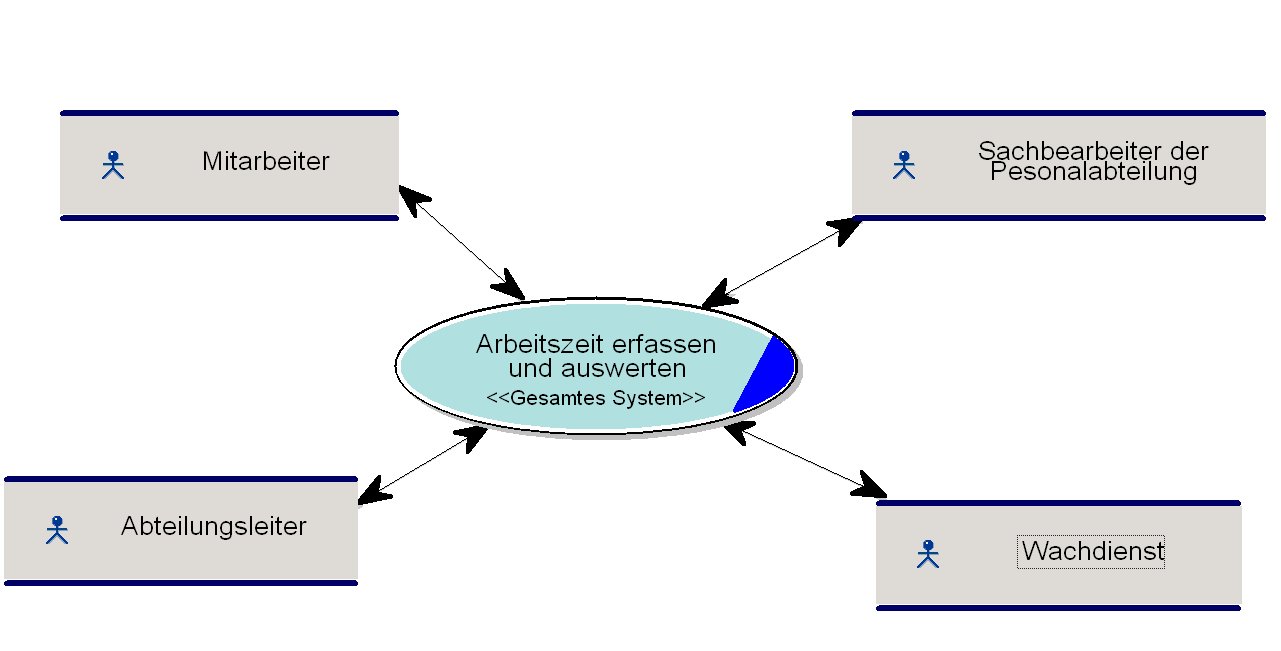
\includegraphics[scale=0.4]{Kontextdiagramm.PNG}
\end{center}

\chapter*{Aufgabe 5: Grobes Anwendungsfalldiagramm}
\setcounter{section}{0}
\addtocounter{chapter}{1}
\addcontentsline{toc}{chapter}{Aufgabe 5: Grobes Anwendungsfalldiagramm}

\begin{center}
	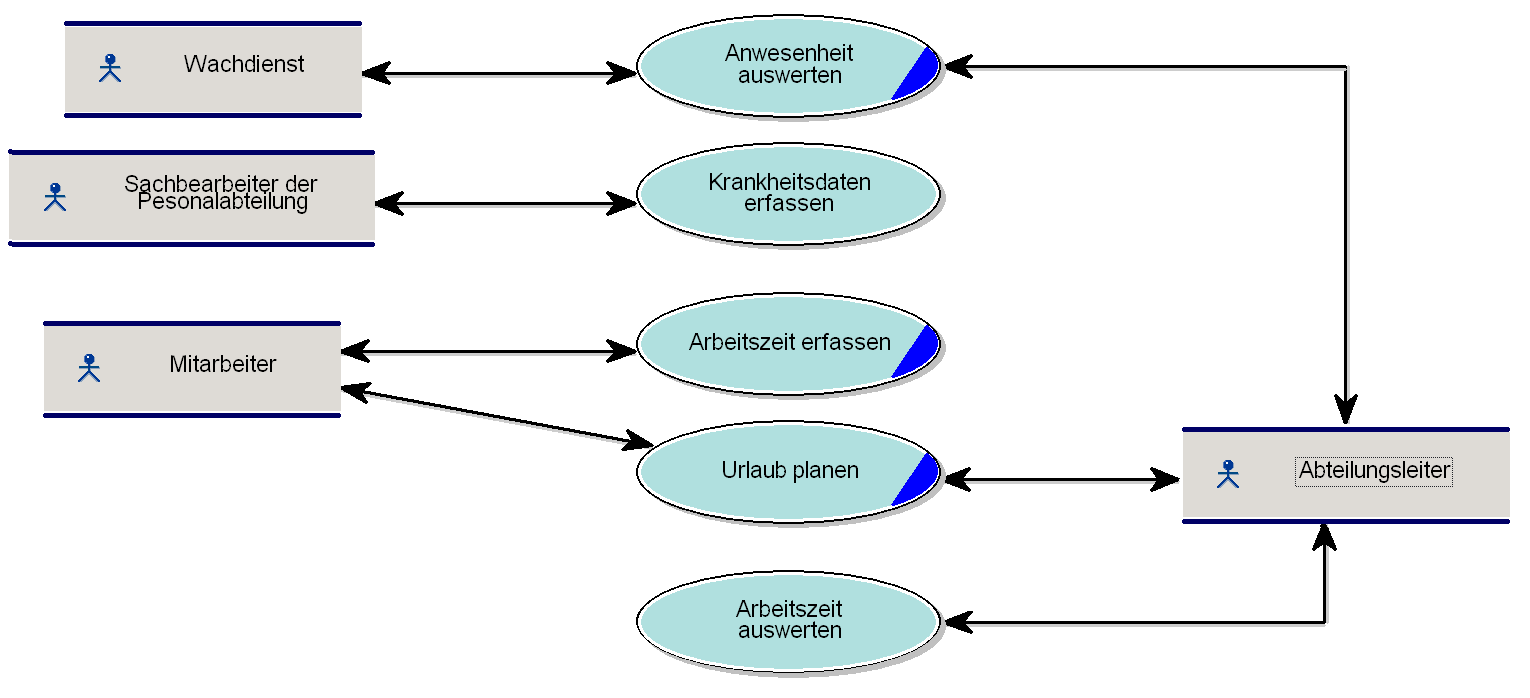
\includegraphics[width=0.9\linewidth]{GrobesAnwendungsfalldiagramm.PNG}
\end{center}


\chapter*{Aufgabe 6: Detailliertes Anwendungsfalldiagramm von Urlaub planen}
\setcounter{section}{0}
\addtocounter{chapter}{1}
\addcontentsline{toc}{chapter}{Aufgabe 6: Detailliertes Anwendungsfalldiagramm von Urlaub planen}

\begin{center}
	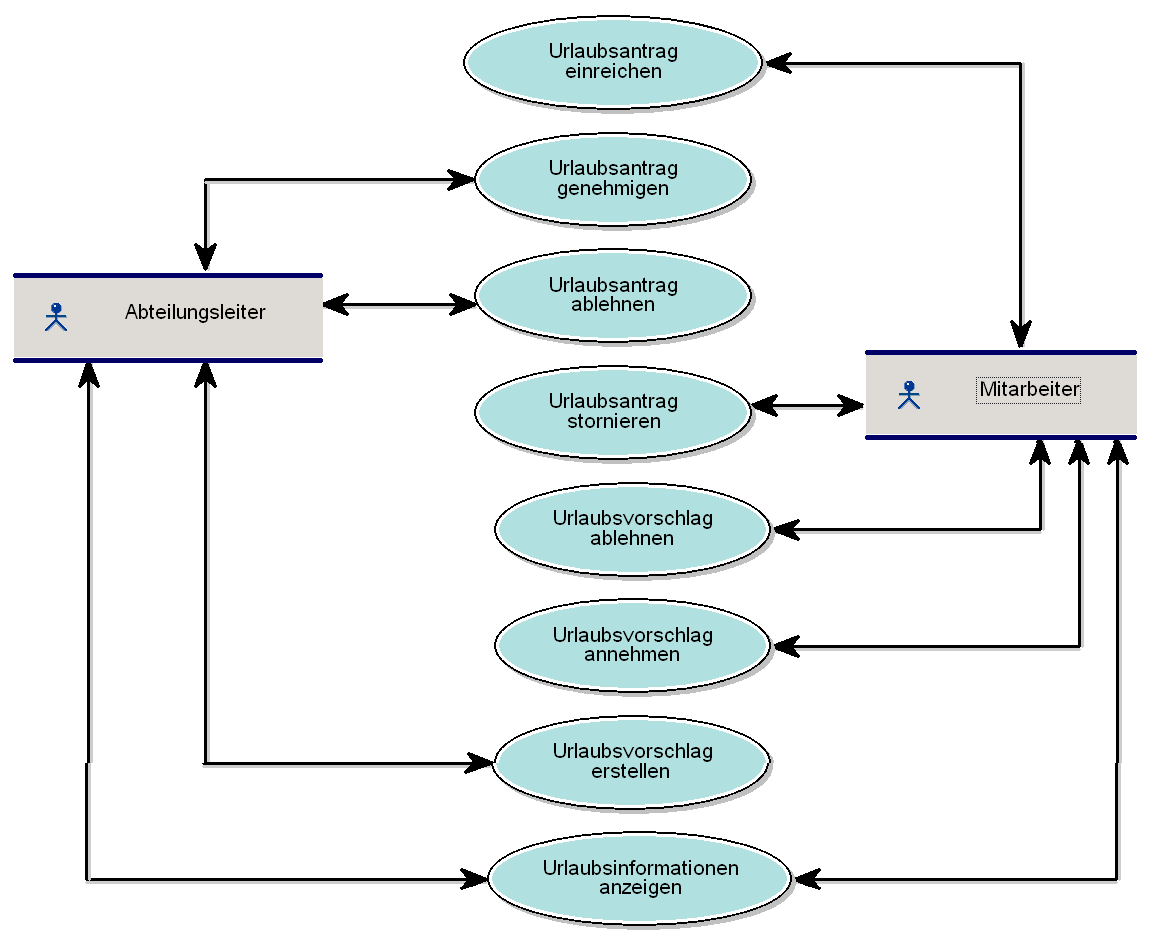
\includegraphics[width=0.9\linewidth]{UrlaubPlanen_AWF.PNG}
\end{center}

\chapter*{Aufgabe 7: Anwendungsfallbeschreibung}
\setcounter{section}{0}
\addtocounter{chapter}{1}
\addcontentsline{toc}{chapter}{Aufgabe 7: Anwendungsfallbeschreibung}

\section{Jonatan: Urlaub einreichen}

\subsection{Textliche Beschreibung}

\subsubsection{Kurzbeschreibung}

Ein Mitarbeiter reicht einen Urlaubsantrag ein.

\subsubsection{Akteur}

Mitarbeiter

\subsubsection{Vorbedingungen}

\begin{itemize}
\item Urlaubsantrag
\end{itemize}

Urlaubsantrag =
\begin{itemize}
\item[] MA\_ID
\item[+] Urlaubs\_ID
\item[+] Zeitraum
\end{itemize}

Zeitraum = 
\begin{itemize}
\item[] Start-Datum
\item[+] End-Datum
\end{itemize}

\subsubsection{Nachbedingungen}
\begin{itemize}
\item Urlaubsantrag ist im System gespeichert
\end{itemize}

\subsubsection{Trigger}
\begin{itemize}
\item Urlaubsantrag stellen
\end{itemize}

\subsubsection{Szenarios}

\paragraph{Hauptszenario:} Mitarbeiter gibt validen Urlaubsantrag ein.
\begin{enumerate}
\item Mitarbeiter möchte Urlaubsantrag stellen
\item Mitarbeiter gibt Urlaubseintrag in System ein
\item System überprüft Urlaubsantrag
\item System trägt Urlaubseintrag in Urlaubsinformationen des Mitarbeiters ein
\end{enumerate}

\paragraph{Alternativszenario:} Mitarbeiter gibt keinen validen Urlaubsantrag ein.
\begin{enumerate}
\item Mitarbeiter möchte Urlaubsantrag stellen
\item Mitarbeiter gibt Urlaubseintrag in System ein \label{jo-alt-back}
\item System überprüft Urlaubsantrag
\item Zurück zu \ref{jo-alt-back}.
\end{enumerate}

Urlaubseintrag=
\begin{itemize}[label=+]
\item[] Urlaubs\_ID
\item Zeitraum
\item Status
\end{itemize}

\subsubsection{Weiterführende Informationen}
keine

\subsection{Aktivitätsdiagramm}

\begin{center}
	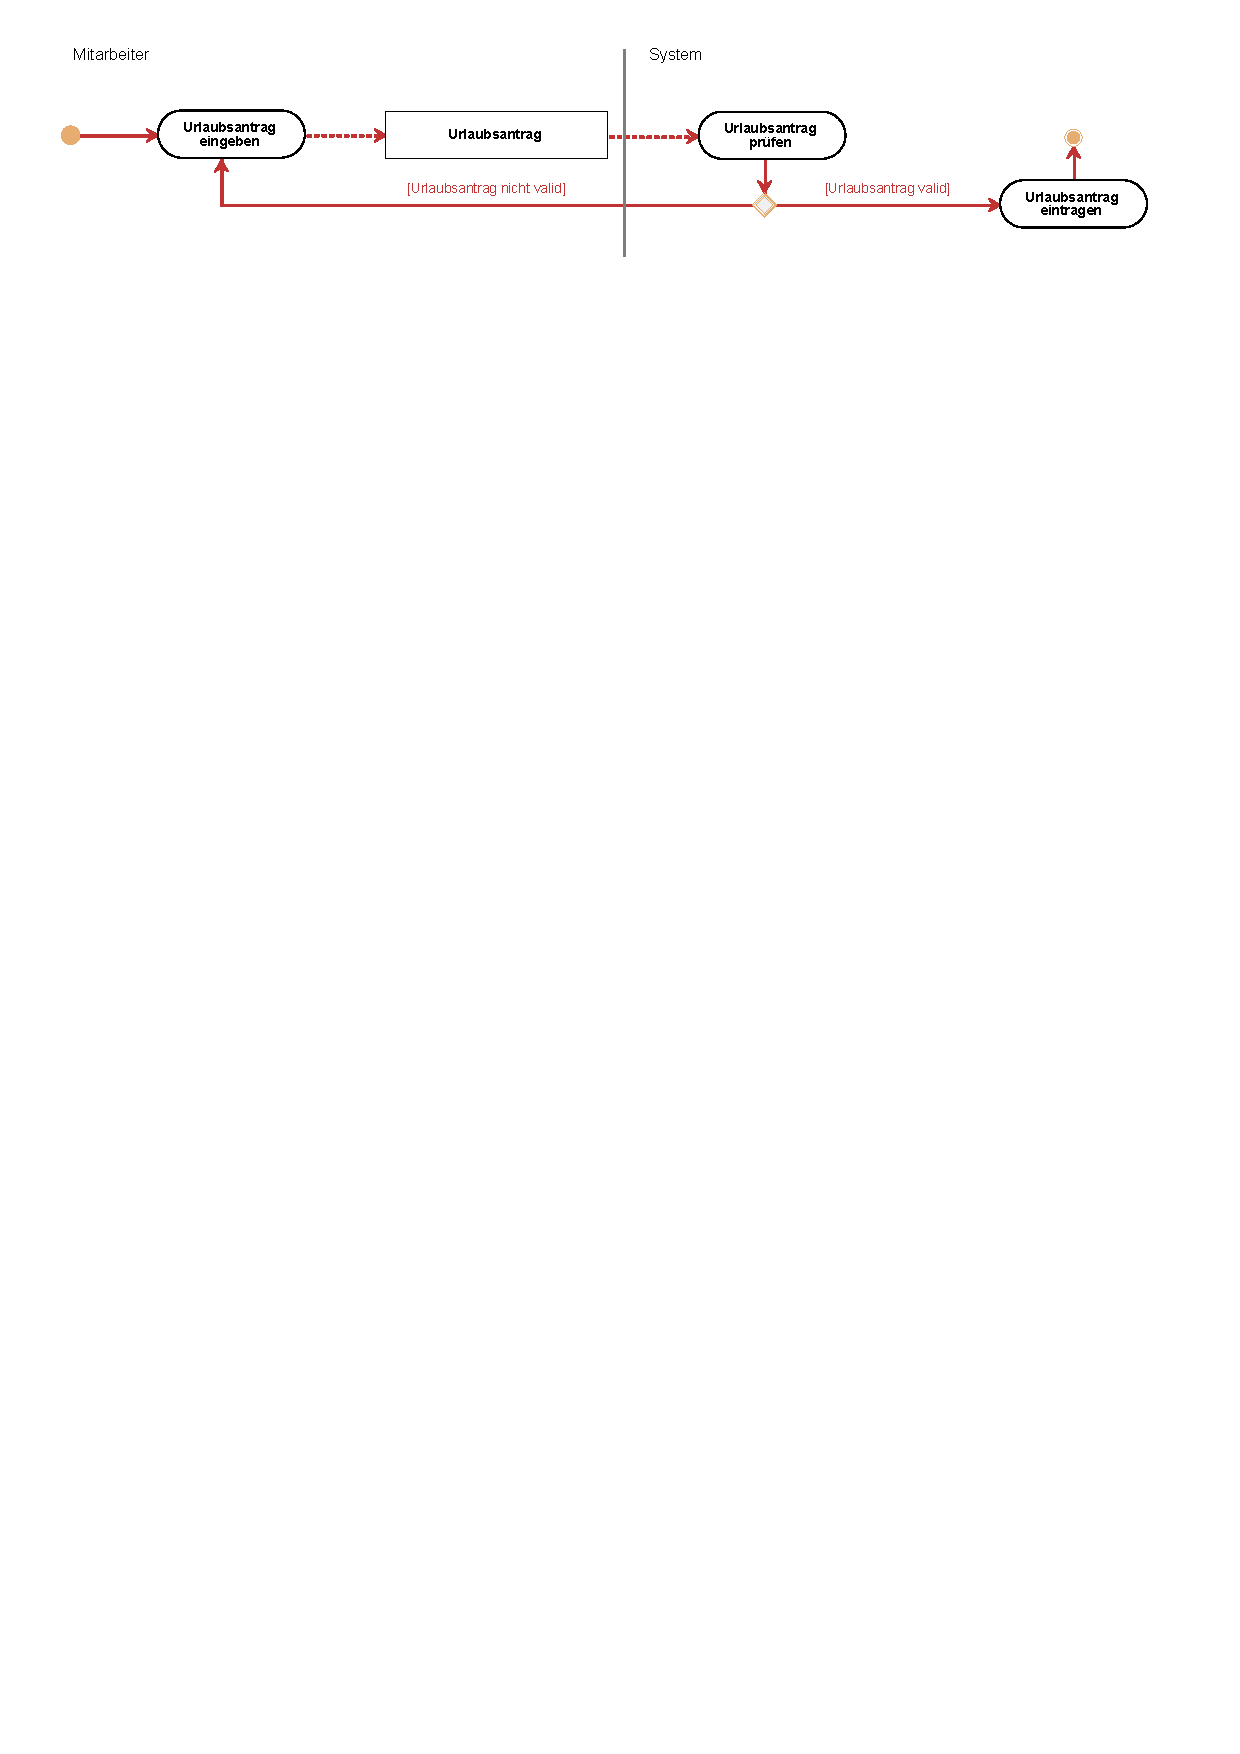
\includegraphics[width=0.9\linewidth]{Urlaub_einreichen.pdf}
\end{center}

\subsection{Satzschablonen}
Die Funktion „Urlaub einreichen“…
\begin{itemize}
\item muss einen eingegebenen Urlaubsantrag erfassen.
\item muss fähig seinen einen erfassten Urlaubsantrag zu prüfen.
\item muss fähig sein einen Urlaubseintrag in die Datenbank einzutragen.
\item muss dem Mitarbeiter die Möglichkeit bieten bei einem nicht validen Urlaubsantrag den Urlaubsantrag erneut einzugeben.
\item soll die Möglichkeit bieten dem Mitarbeiter ausreichend Feedback bezüglich der Validität des Urlaubseintrags zu geben.
\end{itemize}

\section{Simon: Urlaubsvorschlag annehmen}

\subsection{Textliche Beschreibung}

\subsubsection{Kurzbeschreibung}
Ein Mitarbeiter nimmt einen vorgeschlagenen Urlaub an.

\subsubsection{Akteur}
\begin{itemize}
	\item System
	\item Mitarbeiter
\end{itemize}

\subsubsection{Vorbedingungen}
\begin{itemize}
	\item Urlaubs ID
\end{itemize}

\subsubsection{Nachbedingungen}
\begin{itemize}
	\item Urlaub eingetragen
	\item Alternativ Eintragung wird abgebrochen
\end{itemize}

\subsubsection{Trigger}
Wunsch den Urlaubsvorschlag anzunehmen

\subsubsection{Szenarios}
\paragraph{Hauptszenario:}
Urlaubsvorschlag liegt vor und Mitarbeiter nimmt diesen mit einer gültigen Urlaubs ID an.

\begin{enumerate}
	\item Mitarbeiter bekommt Urlaubsinformationen angezeigt
	\item Mitarbeiter gibt die Urlaubs ID an um den Urlaubsvorschlag anzunehmen
	\item Urlaubs ID wird an das System übermittelt
	\item System prüft ob Urlaubs ID gültig ist
	\item System trägt Urlaub als angenommen ein
\end{enumerate}



\paragraph{Alternativszenario:}
Urlaubsvorschlag liegt vor und Mitarbeiter nimmt diesen mit einer ungültigen Urlaubs ID an.

\begin{enumerate}
	\item Mitarbeiter bekommt Urlaubsinformationen angezeigt
	\item Mitarbeiter gibt die Urlaubs ID an um den Urlaubsvorschlag anzunehmen
	\item Urlaubs ID wird an das System übermittelt
	\item System prüft ob Urlaubs ID gültig ist
	\item Mitarbeiter bekommt erneut die Möglichkeit die Urlaubs ID einzugeben
\end{enumerate}


\subsubsection{Weiterführende Informationen}
Urlaub gilt als angenommen

\subsection{Aktivitätsdiagramm}

\begin{center}
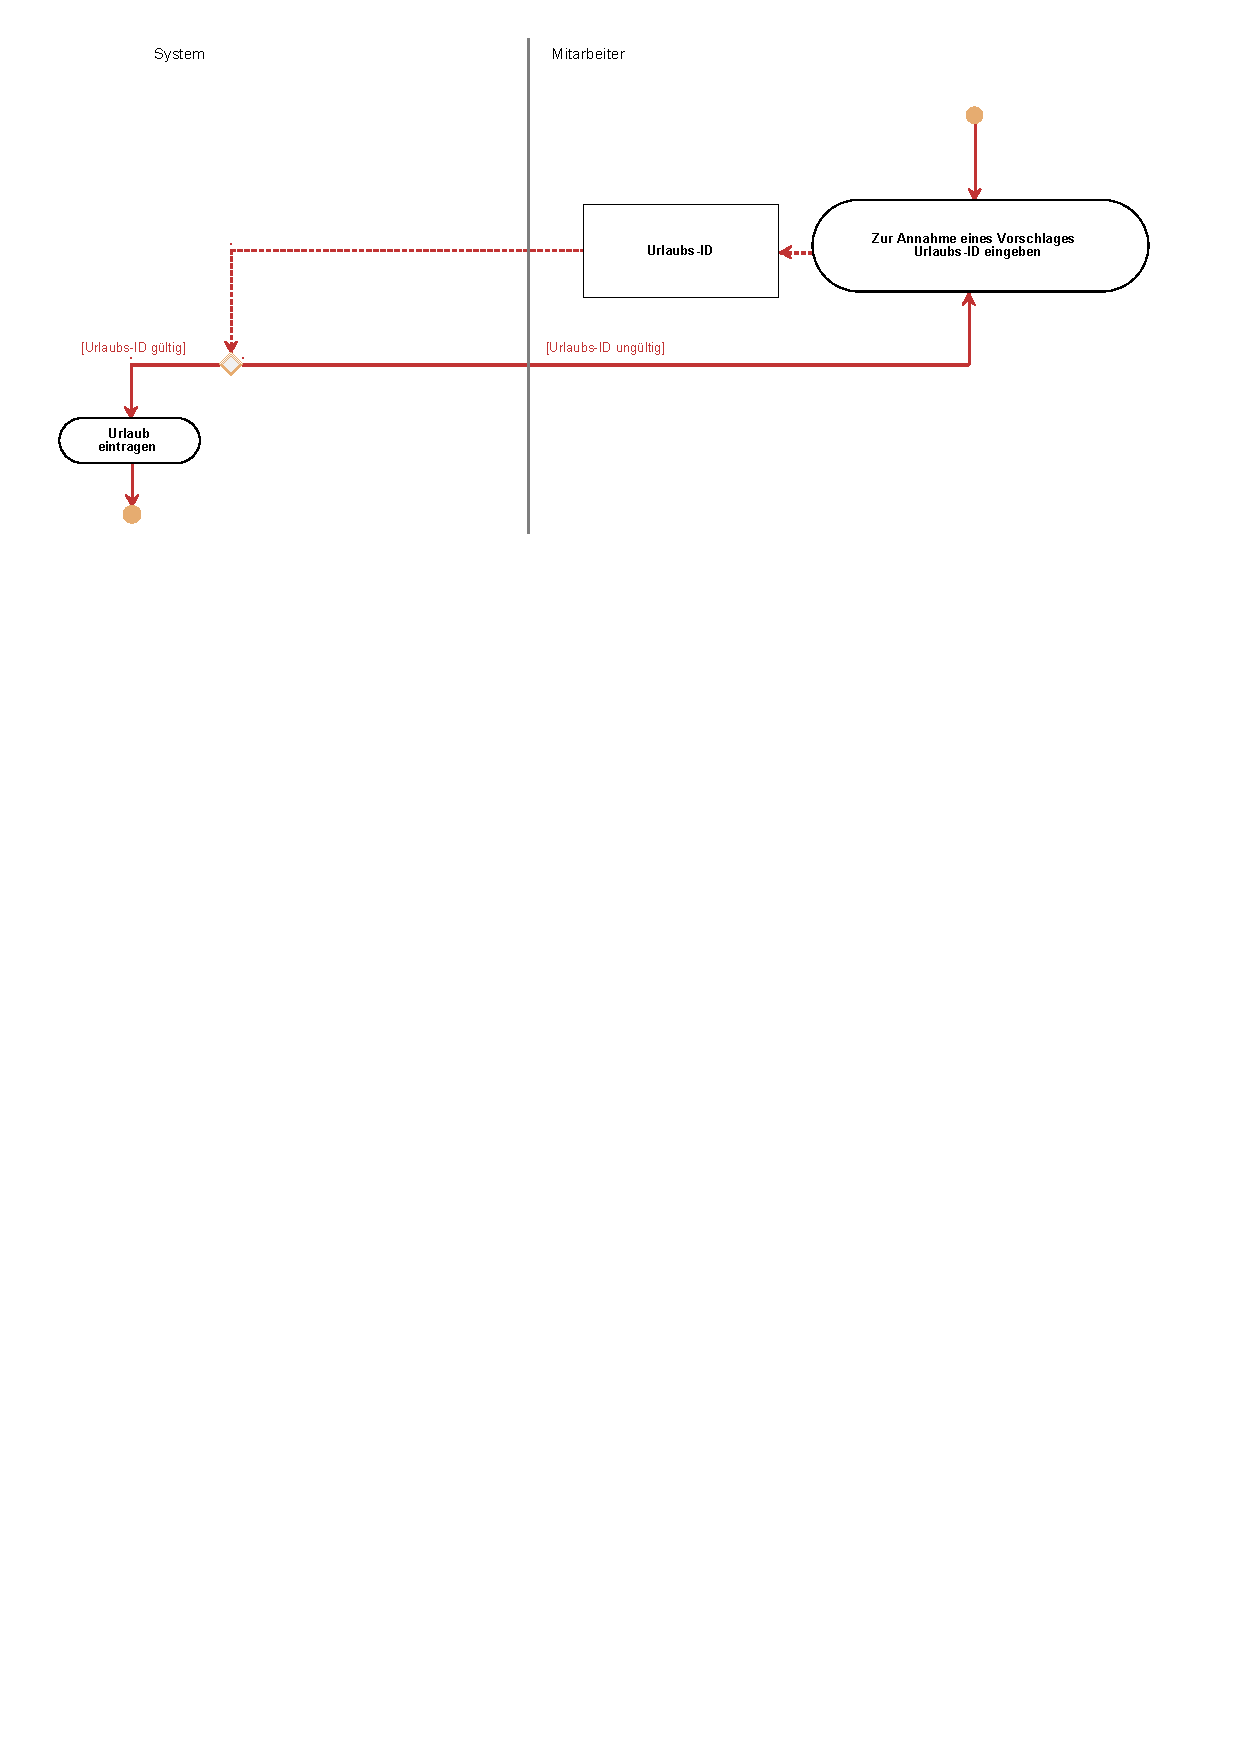
\includegraphics[width=0.9\linewidth]{Urlaubsvorschlag_annehmen.pdf}
\end{center}

\subsection{Satzschablonen}
Die Funktion Urlaubsvorschlag annehmen sollte folgende Aufgaben erledigen:
\begin{itemize}
	\item Entscheidung ob eine Urlaubs ID gültig ist oder nicht
	\item Eintragung eines Urlaubes als angenommen
	\item Dem Mitarbeiter soll die Möglichkeit gegeben werden, dass er nach einer falschen Eingabe der Urlaubs ID, erneut die ID eingeben kann.
\end{itemize}

\section{Ragnar: Urlaubsvorschlag ablehnen}

\subsection{Textliche Beschreibung}
 
\subsubsection{Kurzbeschreibung}
Ein Mitarbeiter lehnt einen Urlaubsvorschlag an.
\subsubsection{Akteur}
\begin{itemize}
\item System
\item Mitarbeiter
\end{itemize}
\subsubsection{Vorbedingungen}
\begin{itemize}
\item Urlaubs ID
\end{itemize}

\subsubsection{Nachbedingungen}
\begin{itemize}
\item Urlaub abgelehnt
\end{itemize}
\subsubsection{Trigger}
Wunsch den Urlaubsvorschlag ablehnen

\subsubsection{Szenarios}
\paragraph{Hauptszenario:}Urlaubsvorschlag liegt vor und Mitarbeiter lehnt diesen mit einer gültigen Urlaubs ID ab.
\begin{enumerate}
	\item Mitarbeiter bekommt Urlaubsinformationen angezeigt
	\item Mitarbeiter gibt die Urlaubs ID an um den Urlaubsvorschlag ablehnen
	\item Urlaubs ID wird an das System übermittelt
	\item System prüft ob Urlaubs ID gültig ist
	\item System trägt Urlaubs als abgelehnt ein
\end{enumerate}

\paragraph{Alternativszenario:}Urlaubsvorschlang liegt vor und Mitarbeiter lehnt diesen mit einer ungültigen Urlaubs ID ab.
\begin{enumerate}
	\item Mitarbeiter bekommt Urlaubsinformationen angezeigt
	\item Mitarbeiter gibt die Urlaubs ID an um den Urlaubsvorschlag ablehnen
	\item Urlaubs ID wird an das System übermittelt
	\item System prüft ob Urlaubs ID gültig ist
	\item Mitarbeiter bekommt erneut die Möglichkeit die Urlaubs ID einzugeben 
\end{enumerate}


\subsubsection{Weiterführende Informationen}
Urlaub gilt als abgelehnt

\subsection{Aktivitätsdiagramm}

\begin{center}
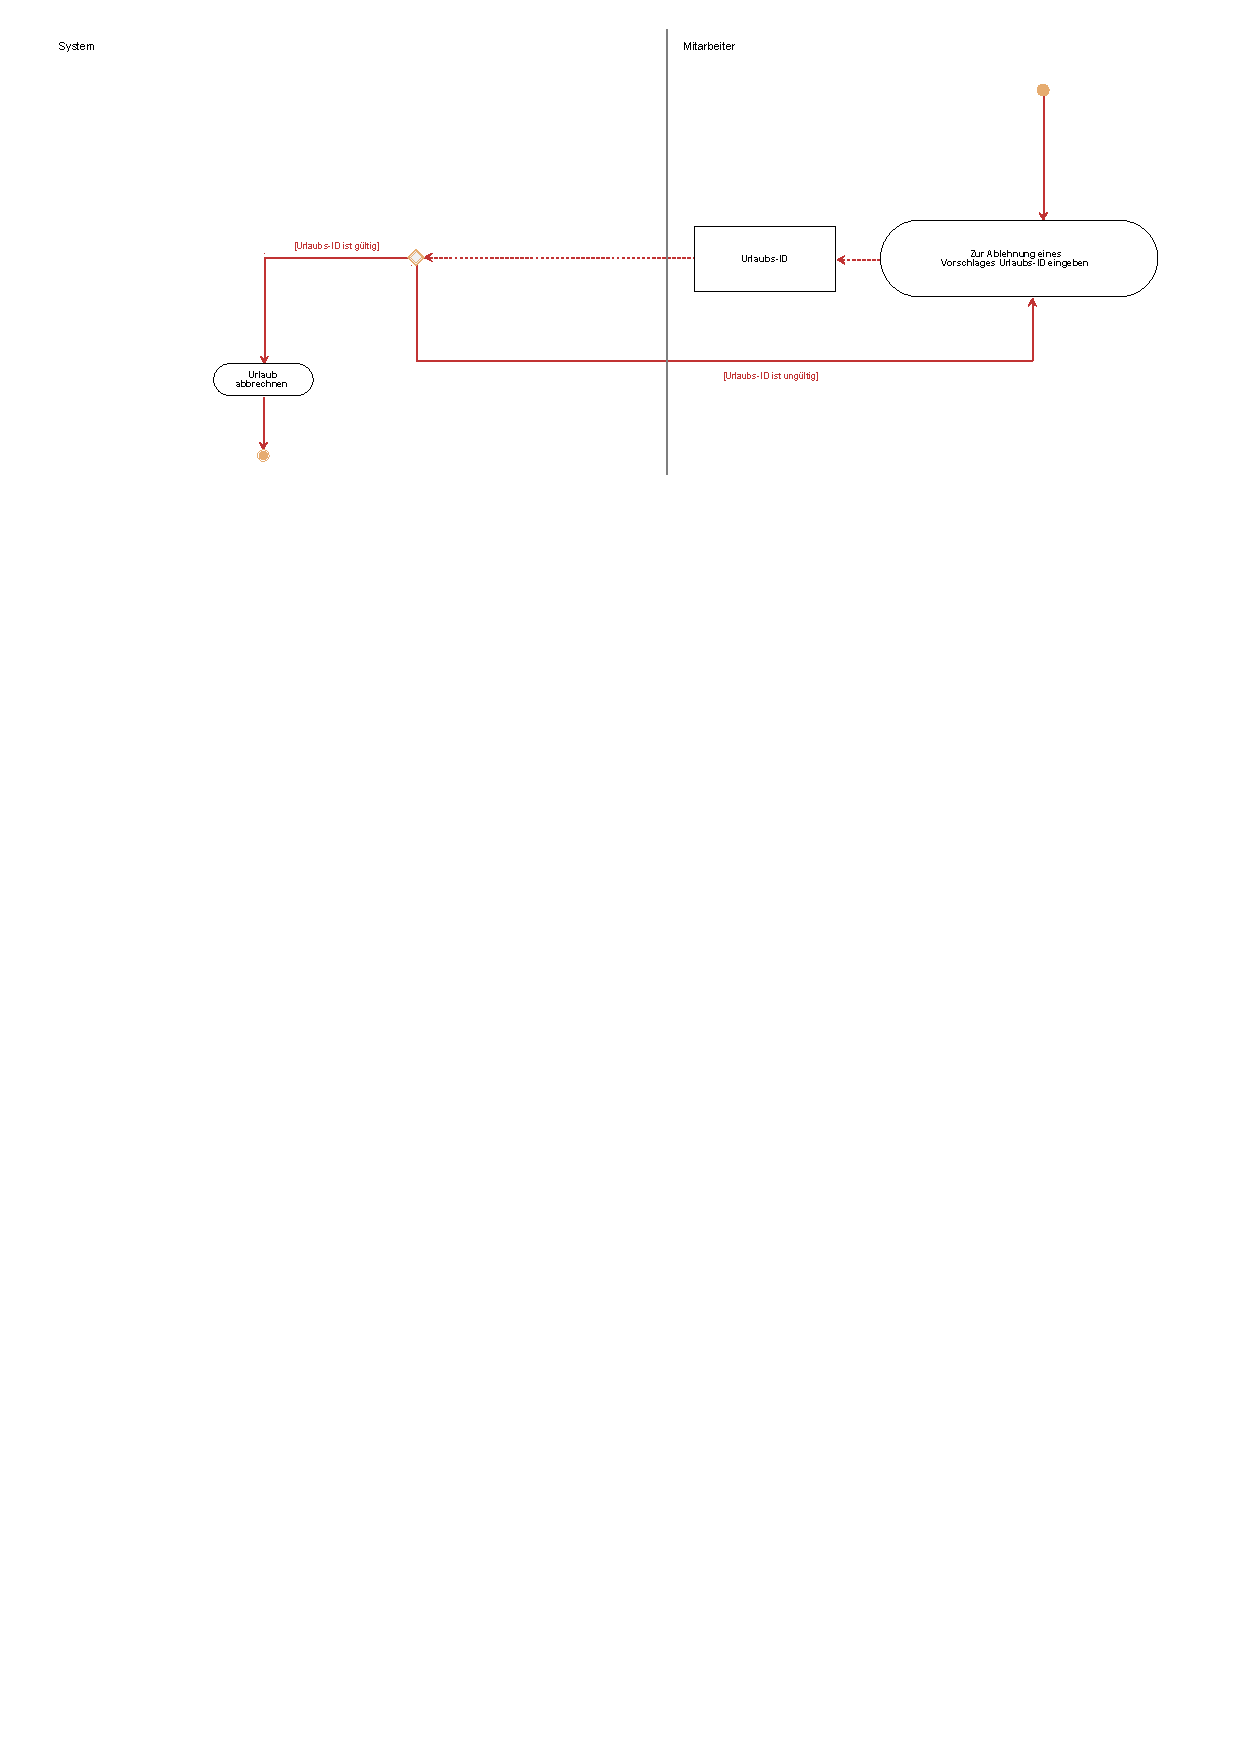
\includegraphics[width=0.9\linewidth]{Urlaubsvorschlag_ablehnen.pdf}
\end{center}

\subsection{Satzschablonen}
Die Funktion Urlaubsvorschlag ablehnen sollte folgende Aufgaben erledigen:
\begin{itemize}
	\item Entscheidung ob eine Urlaubs ID gültig ist oder nicht
	\item Eintragung eines Urlaubes als abgelehnt
	\item Dem Mitarbeiter soll die Möglichkeit gegeben werden, dass er nach falschen Eingabe der Urlaubs ID, erneut die ID eingeben kann.
\end{itemize}
\section{Raphael: Urlaub stornieren}
\subsection{Textliche Beschreibung}
\subsubsection{Kurzbeschreibung}
Ein Mitarbeiter storniert Urlaub.
\subsubsection{Akteur}
Mitarbeiter
\subsubsection{Vorbedingungen}
\begin{itemize}
    \item Urlaubs\_ID
\end{itemize}
\subsubsection{Nachbedingungen}
\begin{itemize}
    \item Urlaub wurde aus dem System ausgetragen
\end{itemize}
\subsubsection{Trigger}
\begin{itemize}
    \item Urlaub stornieren
\end{itemize}

\subsubsection{Szenarios}
\paragraph{Hauptszenario:}

\begin{enumerate}
    \item Mitarbeiter möchte Urlaub stornieren
	\item Mitarbeiter gibt gültige Urlaubs\_ID ein
	\item System prüft Urlaubs\_ID
	\item System prüft ob Urlaubszeitraum in der Zukunft liegt
	\item System entfernt Urlaubseintrag aus der Datenbank
\end{enumerate}

\paragraph{Alternativszenario:}

\begin{itemize}
    \item Mitarbeiter gibt ungültige Urlaubs\_ID ein:
    \begin{enumerate}
    	\item Mitarbeiter möchte Urlaub stornieren
    	\item Mitarbeiter gibt Urlaubs\_ID ein \label{rp-inv-uid}
    	\item System prüft Urlaubs\_ID
    	\item Zurück zu \ref{rp-inv-uid}
    \end{enumerate}
    
    \item Urlaub liegt in der Vergangenheit:
     \begin{enumerate}
    	\item Mitarbeiter möchte Urlaub stornieren
    	\item Mitarbeiter gibt Urlaubs\_ID ein \label{rp-past}
    	\item System prüft Urlaubs\_ID
    	\item System prüft ob Urlaubszeitraum in der Zukunft liegt
    	\item Zurück zu \ref{rp-past}
    \end{enumerate}   
\end{itemize}

\subsubsection{Weiterführende Informationen}
Keine

\subsection{Aktivitätsdiagramm}

\begin{center}
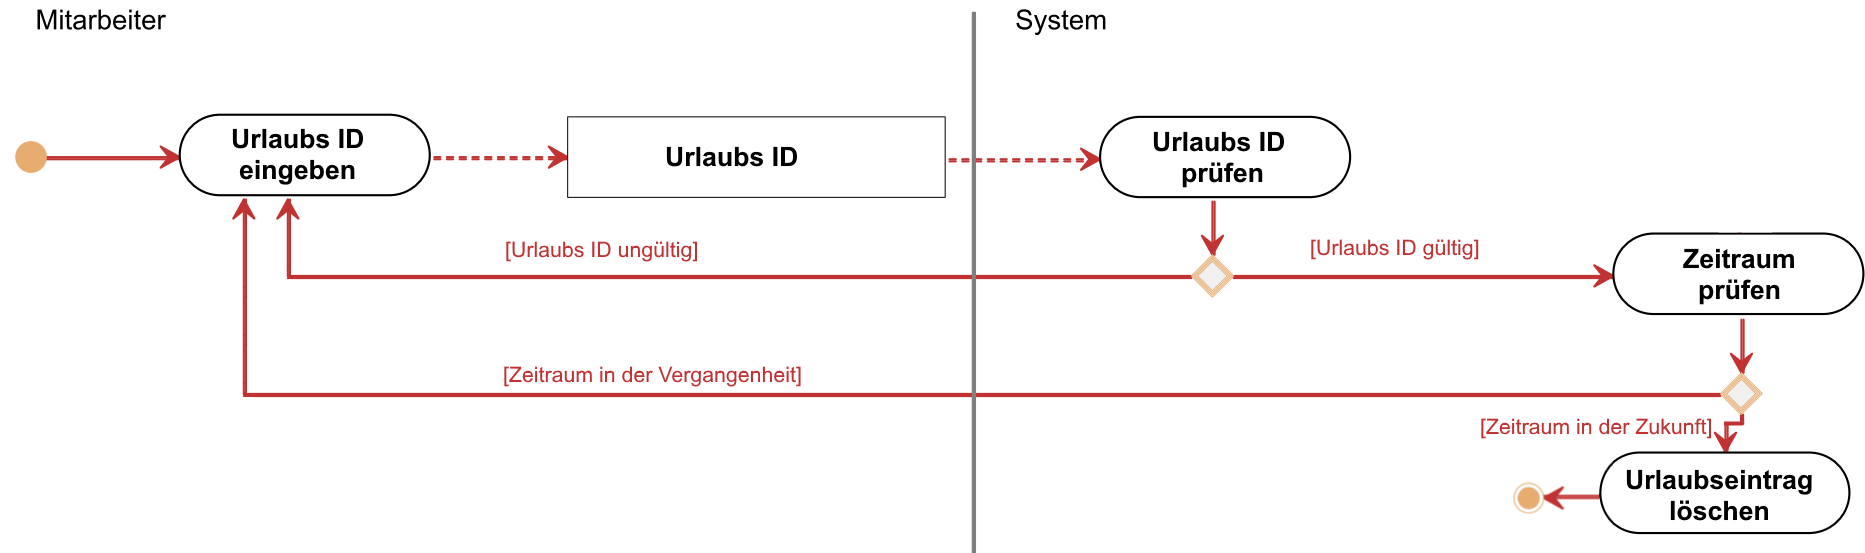
\includegraphics[width=0.9\linewidth]{Urlaub_stornieren.png}
\end{center}

\subsection{Satzschablonen}
Die Funktion „Urlaub stornieren“...
\begin{itemize}
    \item muss fähig sein einen Urlaubseintrag anhand einer gültigen Urlaubs\_ID aus der Datenbank zu löschen.
    \item muss Gültigkeit eines Urlaubseintrags erkennen.
    \item soll dem Mitarbeiter die Gültigkeit seiner Anfrage zurückgeben.
\end{itemize}

\chapter*{Aufgabe 8: Zustandsdiagramm Urlaubsantrag}
\setcounter{section}{0}
\addtocounter{chapter}{1}
\addcontentsline{toc}{chapter}{Aufgabe 8: Zustandsdiagramm Urlaubsantrag}

\begin{center}
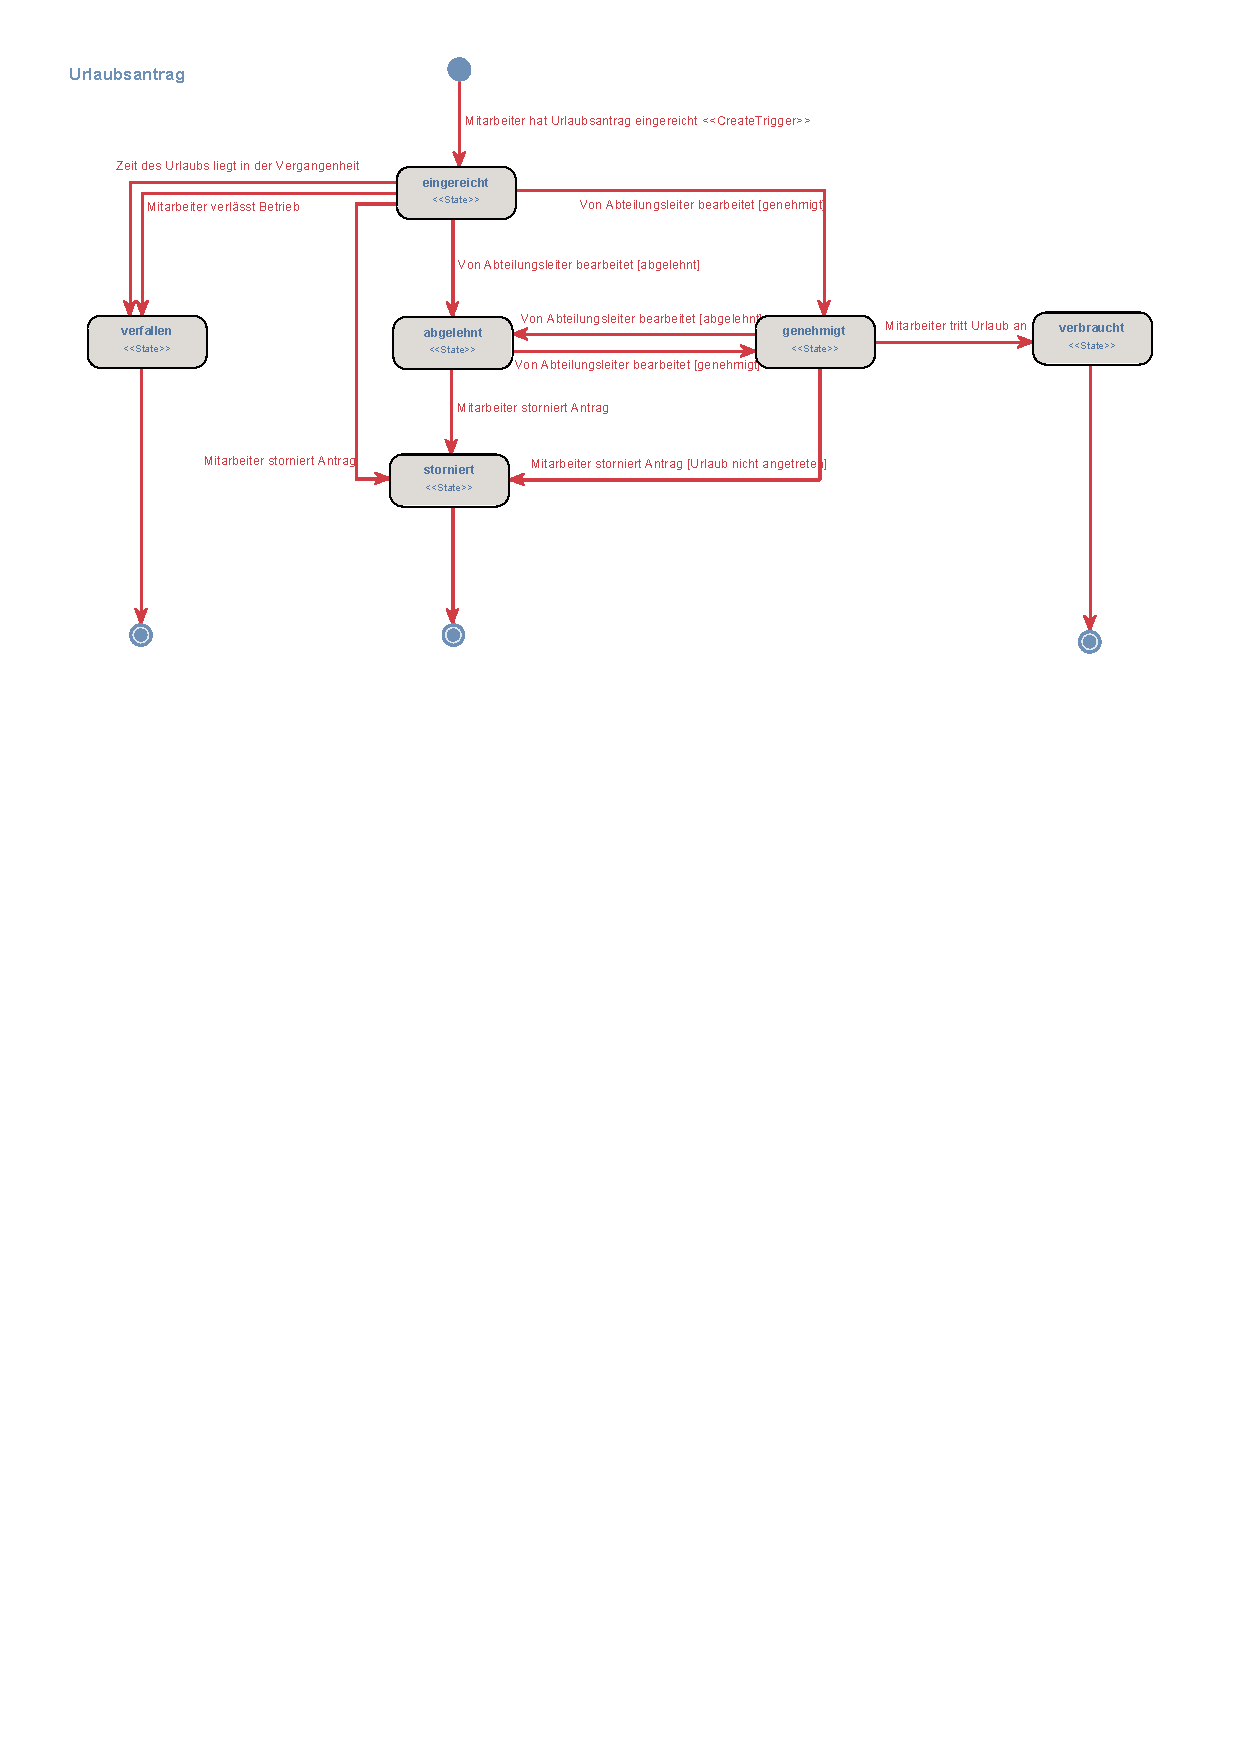
\includegraphics[width=0.95\linewidth]{Aktivitaet_Urlaubsantrag}
\end{center}

\chapter*{Aufgabe 9: ERM}
\setcounter{section}{0}
\addtocounter{chapter}{1}
\addcontentsline{toc}{chapter}{Aufgabe 9: ERM}

\chapter*{Aufgabe 10: Glossar}
\setcounter{section}{0}
\addtocounter{chapter}{1}
\addcontentsline{toc}{chapter}{Aufgabe 10: Glossar}

\begin{tabular}{L{0.3} L{0.7}}
Ablehnung (bei Erfassung der Anwesenheit)					&	Text mit Grund der Ablehnung.				\\
Status (Urlaubseintrag)					&	eingereicht / abgelehnt / genehmigt / storniert / verfallen / verbraucht (basierend auf Urlaubsantrag und Urlaubsvorschlag).				\\
*\_ID					&	Ein eindeutiger Schlüssel (Zahl).				\\
Gültigkeit					&	gültig / nicht gültig				\\
%					&					\\
\end{tabular}

%\printbibliography
 
\end{document}